\documentclass[conference]{IEEEtran}
\IEEEoverridecommandlockouts
% The preceding line is only needed to identify funding in the first footnote. If that is unneeded, please comment it out.
\usepackage{cite}
\usepackage{amsmath,amssymb,amsfonts}
\usepackage{algorithmic}
\usepackage{graphicx}
\usepackage{textcomp}
\usepackage{xcolor}
\usepackage{makecell}
\def\BibTeX{{\rm B\kern-.05em{\sc i\kern-.025em b}\kern-.08em
    T\kern-.1667em\lower.7ex\hbox{E}\kern-.125emX}}
\begin{document}

\title{Synchronisation des formes d'ondes FBMC/OFDM\\
{\footnotesize \textsuperscript{*}Note: Implémentation des formes d'ondes FBMC avec GNURadio}
}

\author{

\IEEEauthorblockN{Llorente Alexis}
\IEEEauthorblockA{\textit{Etudiant M2 : spécialité système embarqué} \\
\textit{ISEN Brest, 29200}\\
20 Rue Cuirassé Bretagne \\
alexis.llorente@isen-ouest.yncrea.fr}
\and
\IEEEauthorblockN{Pottier Antony}
\IEEEauthorblockA{\textit{Enseignant-Chercheur (Associate Professor)}\\
\textit {Département SEACom} \\
\textit{ISEN Brest, 29200}\\
20 Rue Cuirassé Bretagne \\
antony.pottier@isen-ouest.yncrea.fr}
}

\maketitle

\begin{IEEEkeywords}
  OFDM ,FBMC ,GNURadio ,Disturber ,LTE ,Wifi ,OFDM-OQAM.
\end{IEEEkeywords}

\begin{abstract}
Ce document est un état de l'art de plusieurs recherches portées sur les formes d'onde OFDM et FBMC, l'objectif de ce document est d'identifier la possibilité de l'utilisation des formes d'ondes FBMC dans un milieu maritime et de discuter de l' hypothèse lié à la synchronisation de différents signaux qui arrive sur un seule récepteur issus d'un émetteur et d'un perturbateur. 
\end{abstract}



\section{Introduction}
Le développement des activités humaines dans le monde maritime est source de nombreux signaux. Devant le nombre croissant de signaux sous-marins et n’ayant aucun standard d’utilisation de ces signaux, il est nécessaire qu'ils ne s'interfèrent pas entre eux. Ces dernières années, les communications avec multi-porteuses se sont considérablement développées aux seins de nos technologies sans fils. Celles-ci offre un taux de transmission des données plus élevées. En particulier l'OFDM est l’un des plus connu dans ce domaine. Ces dernières années avec l'apparition de la 4G/5G, les formes d’ondes FBMC (Filter Bank Multi-Carrier) ont été considérés comme une alternative au OFDM (Orthogonal Frequency Division Multiplexing). En effet FBMC offre les moyens de surmonter des limitations connues de l’OFDM en terme d’efficacité spectrale réduite et d’éxigence de synchronisation.

\section{Contexte}

FBMC est une généralisation de l'OFDM, actuellement le schéma de modulation le plus populaire utilisé en LTE et WIFI. Dans cette section nous détaillerons chacune d'entre elles avant de les comparer.

\subsection{Les formes d'onde OFDM}
Le signal OFDM est un standard imaginé dans les années 1960 qui consiste à transmettre une information binaire (une suite de bits, c’est-à-dire des symboles) sur des porteuses différentes, autrement sur des fréquences différentes \cite{b3}.Cette suite binaire est une suite d'impulsion de forme rectangulaire produisant par transformation de fourrier une suite de sinus cardinaux orthogonaux entre eux séparé d'une bande de fréquence $\Delta f$ , en d'autres termes quelles que soit les pulsations $g$ ou $f$ dans l'émission on a toujours : $\langle g,f \rangle = 0$

\begin{figure}[htbp]
\centerline{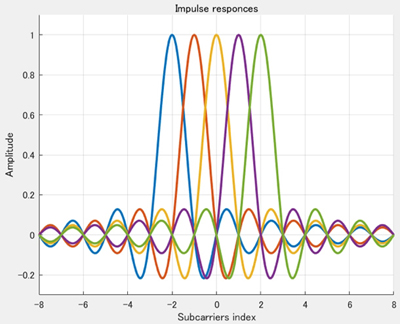
\includegraphics{OFDM_ortho.jpg}}
\caption{Modulation OFDM : orthogonalité des signaux}
\label{OFDM_ortho}
\end{figure}

L'OFDM utilise un Prefixe Cyclique (CP) qui consiste à insérer une copie d’un bloc d’information à transmettre en amont de la trame. Plus clairement, il s’agit de récupérer une partie des informations à transmettre et d’insérer ces informations en début de trame. Le CP joue le rôle de Buffer dans le cas d’une transmission dite à  multi-trajets (plusieurs échos), afin d’éliminer l’interférence entre symboles (ISI).
L'inconvénient principal du CP est que celui ci est redondant. Il n'y a pas de nouvelles informations utile lors de l'utilisation de ce dernier.

\begin{figure}[htbp]
\centerline{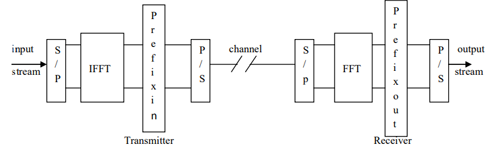
\includegraphics{modemOFDM.png}}
\caption{Modem OFDM}
\label{modemOFDM}
\end{figure}

L'ensemble de la modulation est décrite succinctement dans la Fig.\ref{modemOFDM}. Elle consiste en l'utilisation d'une transformée de fourrier inverse de manière à projeter les symboles sur les sous-porteuses orthogonales de la modulation.


\subsection{Les formes d'onde FBMC}

La forme d'onde FBMC est une amélioration de l'OFDM. Le principal changement se fait dans l'utilisation d'un filtre PPN (PolyPhaseNetwork) qui décale temporellement la valeur réelle et complexe d'une durée d'un demi symbole $\frac{T}{2}$. 
La représentation temporelle et fréquentiel de ces deux formes d'ondes est décrite dans la figure \ref{OFDMFBMCPlan}.

\begin{figure}[htbp]
\centerline{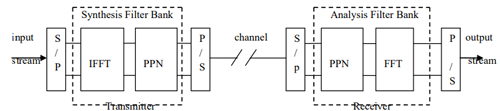
\includegraphics{modemFBMC.png}}
\caption{Modem FBMC}
\label{modemFBMC}
\end{figure}

Les données pour être transmises sont divisées en $M$ différents chemins (sous-porteuse) dans un ensemble de filtres. Le signal résultant $s(k)$ est exprimé par l’équation ci-dessous : 
dans lequel $a_{m,n}$ sont les symboles, $g_{m}$ est le filtre PPN avec n la position temporelle\cite{b4}.
\begin{equation}
s(k) = \sum^{M-1}_{m=0}\sum_{n \in Z}\,a_{m,n}g_{m}(k-\frac{nM}{2})\label{FBMC_equat}
\end{equation}

 
\begin{figure}[htbp]
\centerline{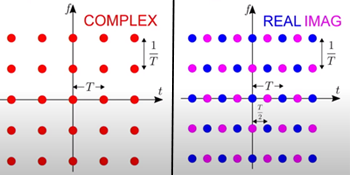
\includegraphics{OFDM_complex.png}}
\caption{Représentation des symboles complexes dans un plan temporel et fréquentiel pour l'OFDM à gauche et le FBMC à droite.}
\label{OFDMFBMCPlan}
\end{figure}

\subsection{Comparaison des formes d'ondes OFDM et FBMC.}

La principale difficulté des formes d'ondes OFDM/FBMC est l'adaptation du signal au canal de propagation ainsi que la synchronisation des données reçu au niveau du récepteur.

Dans un système de radiocommunication classique : un indicatif est $\eta$ l'efficacité spectrale définie par l'équation \eqref{effic_spect}. Celui-ci dans un système idéal doit se rapprocher d'une valeur proche de $1$.

\begin{equation}
\eta = \frac{\beta}{TF}\label{effic_spect}
\end{equation}

Dans le cas de l'OFDM il est nécessaire de rajouter le temps relatif au préfixe cyclique $T_{cp}$ \eqref{effic_spect_OFDM} . $\beta$ est le nombre de bits par symbole. 


\begin{equation}
\eta = \frac{\beta}{(T+T_{cp})F}\label{effic_spect_OFDM}
\end{equation}

Ce que l'on souhaite : c’est un système avec le maximum d’efficacité : 
\begin{itemize}

	\item On souhaite se rapprocher de : $TF\ge1$ (Théorie de Nyquist).
	\item Que les signaux soit bi-orthogonaux c'est à dire qu'ils sont sur des points temps/fréquence différents. Dans ce cas : il n'y a pas d’auto-interférence. 
	\item Arbitrairement bien localisés en temps et en fréquence (c'est à dire que la grille temps/fréquence soit dense). Mathématiquement, ceci signifie que le second moment dans le domaine temporelle et en fréquence doit être inférieur à l’infini \eqref{temp} \eqref{freq}.

\begin{equation}
\int_{- \infty}^{+ \infty} t^{2} \lvert g(t) \rvert ^{2} \, \mathrm{d}t <\infty\label{temp}
\end{equation}

\begin{equation}
\int_{- \infty}^{+ \infty} \xi^{2} \lvert G(\xi) \rvert ^{2} \, \mathrm{d}\xi <\infty\label{freq}
\end{equation}
\end{itemize}
L’OFDM ne respecte pas cette dernière condition \eqref{freq}. 
Il est pas possible de construire un système qui respecte ces trois dernières conditions en même temps. Il est impossible de construire des signaux sur une grille temps fréquence qui respecte les trois conditions ci dessus : : Il s'agit du théorème de "Balian-Low".
Par exemple en OFDM utiliser des pulsations rectangulaire lissé sur les bords détruirait l'orthogonalité des symboles.

%Le FBMC est considéré comme avantageux par rapport à l'OFDM en offrant une efficacité spectrale plus élevée. En raison du filtrage par sous-porteuse, il entraîne un délai de filtrage plus important et nécessite également un traitement OQAM.

Le FBMC fonctionne de manière différente : en modifiants certain de ces 3 derniers points.
En respectant la théorie de Nyquist et possédant une pulsation plus centralisée elle ne se focalise pas sur l'orthogonalité du signal. En effet, FBMC ne cherche pas l’orthogonalité des signaux : pour cette forme d'onde il suffit d’être orthogonal dans l’axe des réels.

On doit s’assurer que les symboles ne rentre pas en interférence. Si un symbole réel rentre en interférence avec un symbole imaginaire ce n’est pas un problème.
On doit donc trouver une forme d'impulsion qui ne génère pas d’interférence entres les symboles.

Par exemple en prenant le point bleu au milieu du diagramme (valeur réelle) sur la figure \ref{OFDMFBMCPlan}, tout les points bleues voisins ne devrait pas être perturbé par les interférences des autres points réelles. Mais nous sommes autorisé à générer des interférences complexes sur ces points. C’est aussi valable à l’inverse pour les points réelles qui ne peuvent être seulement être perturbé par des interférences imaginaires.
Avec ceci on peut utiliser une pulsation avec une énergie plus centralisé en fréquence et en temps. 

\begin{figure}[htbp]
\centerline{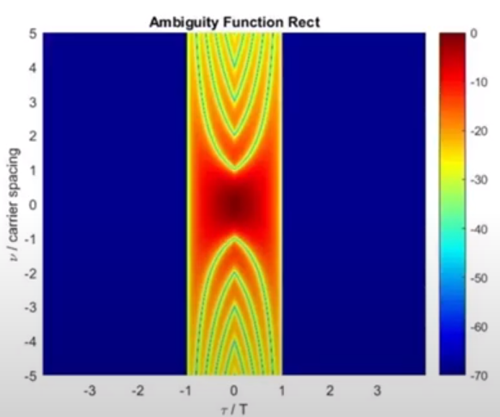
\includegraphics{AmbuigOFDM.png}}
\caption{Fonction d'ambiguïté OFDM}
\label{AmbOFDM}
\end{figure}

La Fig. \ref{AmbOFDM} représente la fonction d'ambiguïté de la fonction rectangle pour l'OFDM. elle permet de déterminer à l'aide de l'énergie du signal si une trame est détectée ou non.
On observe que l'énergie est très localisé en temporel et très large en fréquence.

\begin{figure}[htbp]
\centerline{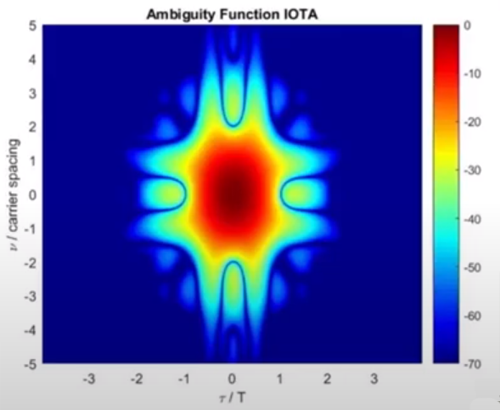
\includegraphics{IOTA.png}}
\caption{Fonction d'ambiguïté IOTA}
\label{IOTA}
\end{figure}

L’utilisation d’un filtre de type IOTA en Fig. \ref{IOTA} est un filtre très populaire en FBMC : parce que ce dernier filtre en fréquence et temporellement et regroupe l'essentiel de l'énergie au milieu de celui ci ce qui n'est pas le cas avec une pulsation rectangulaire type OFDM.


%L'ensemble des informations principales des différentes formes d'ondes sont répertoriés dans le tableau ci-dessous.

%\begin{center}
%    \begin{tabular}{ | c | c | c |}
%      \hline
%      \thead{Comp.} & \thead{OFDM} & \thead{FBMC} \\
%      
%      \hline
%       \makecell{Lobes\\lat.} &  \makecell{Grand (-13dB attenuation)}  & \makecell{Faible
%}  \\
%
%      \hline
%      Sync. &  \makecell{Pour une bonne détection\\ un multiple access \\ interférence (MAI) doit être \\ effectué au niveau du \\recepteur.}  & \makecell{MAI n'est\\ pas néccéssaire\\
%car on connait les\\ pics en fréquence \\ des sous porteuses.
%}  \\
%      \hline
%      CP &  \makecell{CP extension est \\ nécéssaire et réduit \\ l'éfficasité de la \\ bande passante} & \makecell{Non requis
%}  \\
%\hline
%      Cplx. &  \makecell{Faible} & \makecell{Haute
%}  \\
%      \hline
%    \end{tabular}
%  \end{center}

  
\section{Méthode(s) proposée(s)}
Le banc d'essai transmet des trames avec des formes d'impulsions non rectangulaires et se synchronise dans le domaine fréquentiel.

L'ensemble du banc d'essai s'effectue sur le logiciel GNURadio 3.7.15 avec le Framework Qt4 sous GNU/Linux Ubuntu 16.04. 
Elle peut être utilisé avec du matériel Hardware : HackRF ,BladeRF ou USRPs N210 / Intel i7-4770 ou en simulation. Pour notre cas nous simulerons le modem auquel on introduira par la suite perturbation extérieure.

\subsection{Chaine d'émission d'un message}

Le graphique représenté ci dessous sur la Fig.~\ref{EmissionFBMC} représente la chaine d'émission d'un émetteur modulant un signal FBMC : les informations venant dans le bloc "Carrier Allocator" sont issus d'un flux UDP simulé sur la loopback du PC de test. Le Carrier Allocator : Ce dernier transforme les valeurs binaires en symboles OQAM, le FBMC OQAM Block celui traite la séparation entre les symboles entre partie imaginaire et réelle. Il sort deux valeurs ou vecteur et donne une valeur réelle et un vecteur imaginaire : sur ce niveau on sépare la donnée en deux. Ensuite nous avons la IFFT qui se charge de basculer l'ensemble vers le domaine temporel puis le FBMC PPN. C’est une implémentation efficace pour la forme de l'impulsion de la sous porteuse, dans ce block chacune des sous porteuses sont filtrés avec le filtre du type IOTA. On passe donc d'une pulsation rectangulaire à une pulsation plus lissée où l'énergie est concentré au centre de la pulsation. Les symboles étant séparés il est nécessaire de les regrouper dans le même signal ceci est fait avec le block FBMC P2S. La suite est relative au traitement radio.

\begin{figure}[htbp]
\centerline{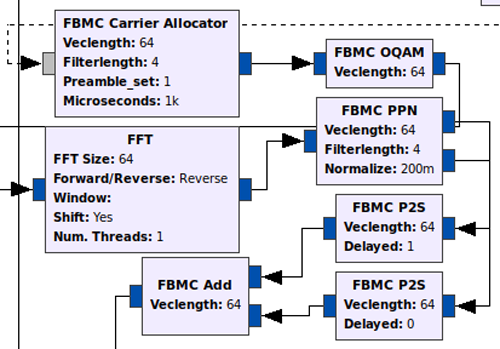
\includegraphics{EmetteurFBMC.png}}
\caption{Chaine d'émission d'un symbole FBMC}
\label{EmissionFBMC}
\end{figure}

\subsection{Chaine de réception d'un message}
Le graphique représenté ci dessous sur la Fig.~\ref{RecepteurFBMC} représente la chaine d'émission d'un émetteur modulant un signal FBMC : Il utilise une synchronisation par fréquence, avec un equaliser sur chaques sous porteuse (On utilise ici Viterbi decoder qui décode à l'aide d'un algorithme de synchronisation)\cite{b2}. Le signal arrive sur deux branches. Un bloc de délais qui gère d’échantillonnage en phase/quadrature (IQ) dans le domaine temporel en parallèle avec le FBMC AFB (Analysis Filter Bank) qui est responsable de la transformation de l'échantillonnage l’IQ vers le domaine fréquentiel : la sortie de ce block est dans le domaine fréquentiel. Ensuite on trouve le FBMC Cross Correlation Function (CCF) qui se charge la corrélation croisée dans le domaine fréquentiel pour la détection des trames, il mesure aussi le symboles avec un offset de timing : donc il ne fait pas que détecter les trames mais il détermine aussi ou les trames commence. Il mesure aussi la fréquence de la porteuse en offset. Cette mesure a besoin d’être corrigé : Donc lorsqu’une trame est détecté il passe dans un bloc le FBMC Frame Extractor qui extrait la trame et délimites chacune d’entre elles. Ensuite les données sont séparé en deux parties individuelles réelle et imaginaire passé dans une FFT puis dans un equaliseur et enfin dans FBMC OQAM recv qui réuni la partie réelle et imaginaire et recréer le symbole pour décoder l’information. Finalement à la fin du diagramme on retrouve l’information initialement émise.


\begin{figure}[htbp]
\centerline{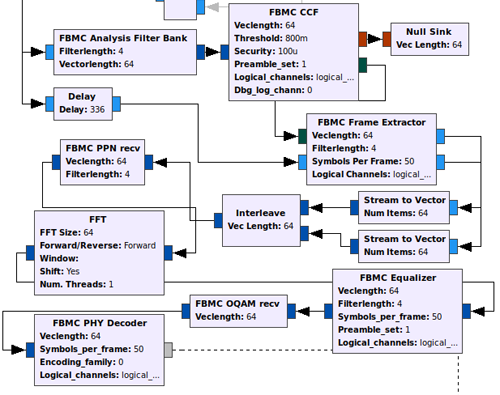
\includegraphics{RecepteurFBMC.png}}
\caption{Chaine de réception d'un symbole FBMC}
\label{RecepteurFBMC}
\end{figure}

\section{Expérimentations et résultats}

\subsection{Objectifs}

L'objectif de l'expérimentation est d'introduire un signal perturbateur (ici un sinus) et d'observer le comportement sur la réception d'un message à l'aide de la synchronisation en fréquence.
Pour se rapprocher du réel entre la chaine de réception et d'émission a été rajouté un bruit gaussien avec une amplitude adapté à l'expérience.

Une description plus précise de l'algorithme de synchronisation en fréquence peut être trouvé en lien bibliographique \cite{b2}.

\subsection{Résultats}
 
 La figure \ref{Resultats} est le résultat d'une simulation, il s'agit d'un spectre FBMC avec 64 sous porteuses au total avec 52 sous porteuse utilisé pour transmettre des données. Et sur le coté droit on a volontairement déactivé 6 sous porteuse ce qui est possible en OFDM aussi mais l’entaille ce sera pas aussi profonde que le FBMC à cause des lobes secondaires. Et dans cette entaille est placé un émetteur en bande étroite. Dans l'expérience il s'agit juste un sinus mais il peut s’agir d’un autre système totalement indépendant l’un l’autre.Ils peuvent coexister en même temps et n’interfèrent pas en même temps l’un l’autre. Le problème avec ce scénario est le fait que on peut pas établir une synchronisation temporelle. Habituellement lorsqu’on a une trame avec une partie donnée et une entête.Pour synchroniser la trame, on effectue une corrélation entre le temps et lorsqu’on reçoit un pic : on détecte une trame. Ce n’est pas possible dans ce scénario parce que dans le meilleur des cas le second système rajoutera un bruit blanc au processus de synchronisation et dans le pire des cas le système FBMC et le système à bande étroite peuvent être corrélés. Dans ce cas on observe un nombre de pics qui ne signifient pas qu’il ont détecté une trame mais que le signal est corrélé et donc peut avoir comme effet de perturber la synchronisation.
 
\begin{figure}[htbp]
\centerline{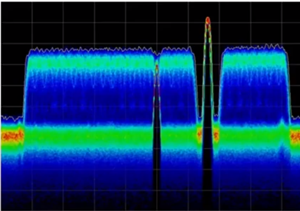
\includegraphics{Resultats.png}}
\caption{Signal FBMC avec perturbateur sinusoïdal.}
\label{Resultats}
\end{figure}


 
Une solution pourrait être de synchroniser non pas dans le domaine temporel mais dans le domaine fréquentiel. Donc la première chose à faire serait de transformer dans le domaine en fréquence : Depuis l’antenne est reçu les échantillons IQ. Ces derniers sont transposés dans le domaine fréquentiel. Pour ne pas interférer avec notre système on ignore tout les sous porteuses utilisé par le perturbateur, dans ce cas nous devrions ignorer les 6 sous porteuses utilisés par le second système . Dans une seconde phase, le signal est corrélé dans le domaine fréquentiel. Puis les bandes de fréquence sont corrélées les unes avec les autres : De cette manière une détection des trames dans le domaine fréquentiel est plus satisfaisante et génère moins d'interférences.

\section{Conclusion}

Le FBMC est considéré comme avantageux par rapport à l'OFDM. Le problème de co-existence de plusieurs systèmes en partie dans le monde sous marin est problématique et les systèmes pourraient s'interférer entre eux. L'ajout d'une synchronisation dans le domaine fréquentiel et l'utilisation du FBMC pourrait répondre à ce problème. Deux système ainsi pourrait co-exister sur une même bande de fréquence grâce à l'implémentation faite dans GNURadio qui pourrait être retranscrite sur un système réel.

\section*{Remerciements}

Mes remerciements vont tout d'abord en direction d'Antony POTTIER pour nous avoir proposé ce sujet. Mais aussi envers Philippe FORJONEL
Enseignant-Chercheur en électronique
aussi de l'équipe SEACom (Systèmes Embarqués, Acoustique et Communications) pour l'aide de la mise en forme de cet article. Je tiens également à remercier mon binôme Alan JAGOT avec qui j'ai travaillé afin de comprendre les enjeux et les ressorts de ce sujet.
%
%\section*{References / Bibliographie}
%
%Une partie de cet article se base majoritairement sur le travail de M.Penner présenté lors de la conférence de la SDRA en 2018 \cite{b1}. Ainsi que sur l'explication de l'algorithme de la synchnositation fréquentiel de l'équipe de C.Thein \cite{b2} et de l'université de Poitier \cite{b3} croisé avec le travail de comparaison OFDM/FBMC de l'université de Dehradun en Inde \cite{b4}.

\begin{thebibliography}{00}
\bibitem{b1} M.Penner ''Adaptive FBMC Real-Time Testbed based on GNU Radio'', June 2018. https://github.com/maxpenner/gr-fbmc
\bibitem{b2} Christoph Thein, Malte Schellmann , Jürgen Peissig 'Analysis of frequency domain frame detection and synchronization in OQAM-OFDM systems' 2014 https://link.springer.com/article/10.1186/1687-6180-2014-83
\bibitem{b3} Université de Poitier : présentation de la forme d'onde OFDM et préfixe cyclique. http://blogs.univ-poitiers.fr/f-launay/tag/spectre/
\bibitem{b4} Bidyalaxmi Devi Tensubam, Nongmaithem Lalleima,Sonika Singh, Ph.D, 
Comparative Analysis of FBMC and OFDM Multicarrier
Techniques for Wireless Communication Networks 
\end{thebibliography}
\vspace{12pt}

\end{document}
